\section{Factorial of a number}
\subsection{Aim}
To calculate the factorial of an 8-bit number

\subsection{Code}
\begin{lstlisting}
ORG 0000H

MOV R0, #5 ; Number to find factorial

MOV A, R0

FACT:
    DEC R0
    CJNE R0, #01, REL ; value of R0 is compared with 1
    JMP stop ; if R0=1, stop execution

REL:
    MOV B, R0
    MUL AB
    JMP FACT

STOP:
    END
\end{lstlisting}

\subsection{Output}
\textbf{Input} 05H (R0)\\
\textbf{Output} 78H (120D) (A)\\
\begin{center}
	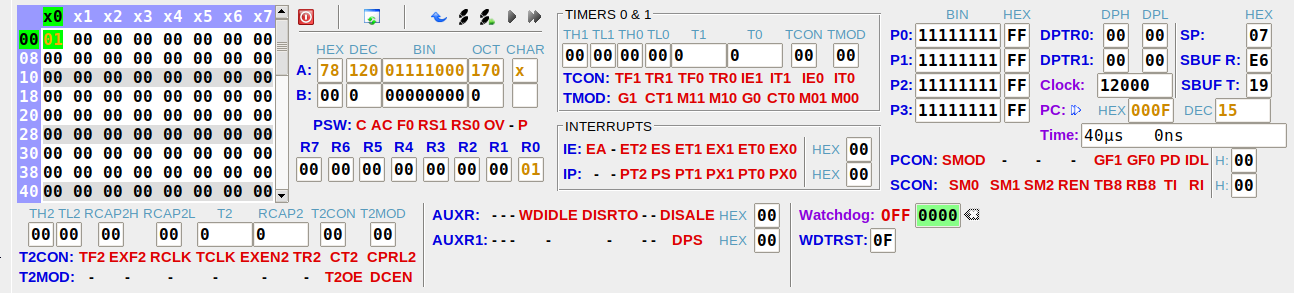
\includegraphics[width=\textwidth]{img/p27.png}
\end{center}


\subsection{Result}
Factorial of a number was found in mcu8051ide